\section{Nombre: Itztlacoliuhqui}  \label{per:itztlacoliuhqui}

\subsection{Descripción:}
Dios de complexión corpulenta, piel blanca y de estatura alta. Tiene unas marcas negras en varias partes del cuerpo como señal de que se rebeló durante la creación del quito sol. Usa una venda en la frente para cubrir la herida causada por la flecha que le devolvió Tonatiuh. Toda la indumentaria que usa para como armadura esta hecha de oro con piedras de esmeraldas incrustadas, tal como la hombrera, el protector de cuello y pecho y los protectores de antebrazos. Porta una capa que se cruza a su cuerpo del lado izquierdo y usa un taparrabos como los que usan los nobles.
\\
\par
De carácter frio e imparcial. Itztlacoliuhqui toma su deber con seriedad y honor. Es un dios de pocas palabras, pero cuando habla acostumbra a ser directo. Prefiere las acciones a las palabras. 
\subsection{Status:}
	\begin{itemize}
		\item Personaje no jugable.
		\item Enemigo jefe.
	\end{itemize}	  
\subsection{Imagen}
Ver figura \ref{fig:diosCastigo}
	\begin{figure}
					\centering
					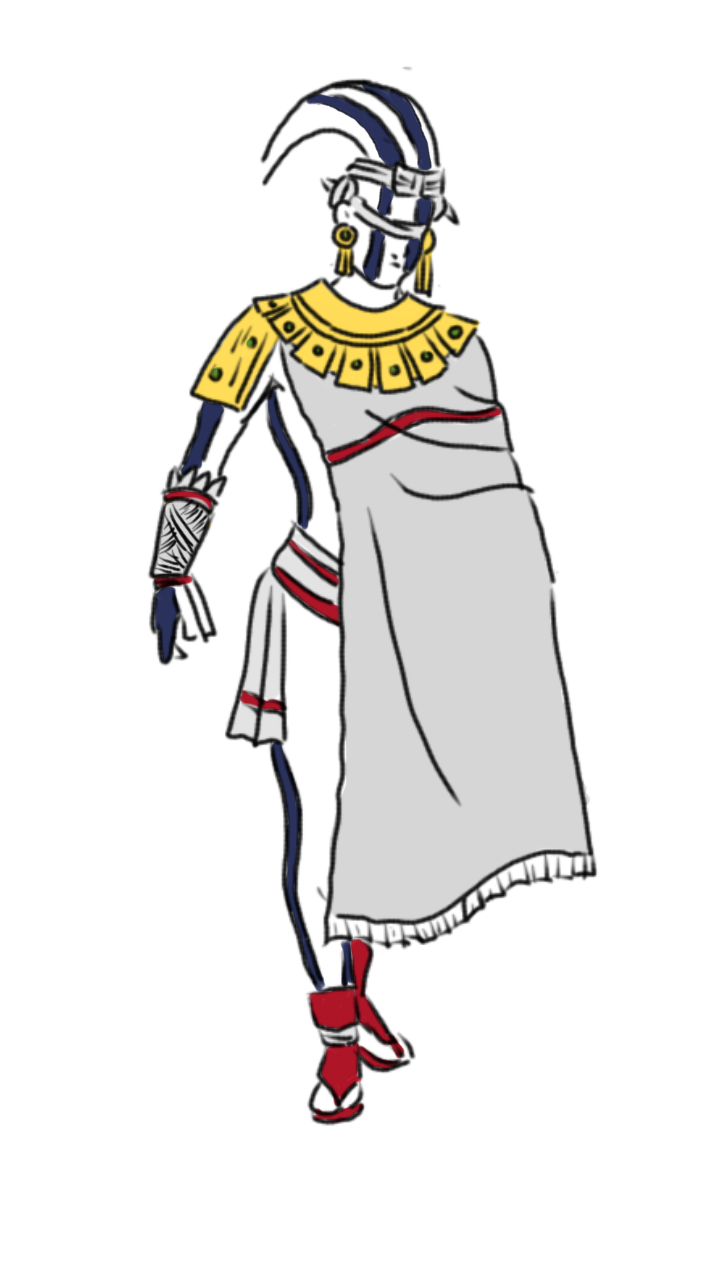
\includegraphics[height=0.3 \textheight]{Imagenes/diosCastigo}
					\caption{Concepto de diseño de Itztlacoliuhqui.}
					\label{fig:diosCastigo}
	\end{figure}
\subsection{Concepto:}
\begin{itemize}
	\item \textbf{Historia antes del juego:}
	En los tiempos anteriores al quinto Sol, el dios del castigo era conocido por el nombre de Tlahuizcalpantecuhtli y se desempeñaba como el dios de la madrugada y de Venus. De actitud alegre y amable, gozaba de una buena relación con los demás dioses; sin embargo, su amabilidad era una pantalla para ocultar la gran soberbia y orgullo que habían dentro de su corazón.
	\\
	\par
	Con la creación del quinto sol, Itztlacoliuhqui se sintió ofendido ante la nueva jerarquía divina pues consideraba que se le había relegado importancia por lo que decide derribar el quinto sol para imponer una nueva jerarquía divina.  Itztlacoliuhqui inicia su rebelión enfrentándose con Tonatiuh, pero es derrotado por éste.  Itztlacoliuhqui es castigado por sus acciones y como marca por su traición su forma y deber cambian, convirtiéndose en el Dios del castigo y siendo asignado como guardián uno de los guardianes del Mictlán.
	\\
	\par
	Como guardián del Mictlán,  Itztlacoliuhqui encuentra una manera de revindicarse en su nuevo rol. Es en el Mictlán donde conoce a Itzpapálotl. Diosa de la que se enamoraría y con quien se casaría.
	\item \textbf{Historia durante el juego:}
	Cuando Itztlacoliuhqui se entera del invasor del inframundo no muestra la más mínima señal de preocupación pues no lo considera una amenaza real, así que decide seguir con la cotidianidad de sus tareas ignorando un poco las ordenes de Mictlantecutli.
	\\
	\par
	Cuando se entera de la caída de Itzpapalotl, el deber deja de tener importancia para él y por primera vez en mucho tiempo Itztlacoliuhqui se deja gobernar por sus emociones. El deseo de recuperar la energía de Itzpapalotl para restaurarla se anteponga a su calma y sentido del honor.
	\\
	\par
	Cuando Itztlacoliuhqui se encuentra a Xolotl y Malinalli, Xolotl trata de convencerlo de que se una a él y a cambio de su ayuda restaurara la energía de Itzpapalotl. El dios del castigo se niega a escuchar a Xolotl y se transforma en un monstruo gigante para destruir a sus enemigos. Al final es derrotado por ella.
	\item \textbf{Relaciones:}
	\begin{itemize}
		\item \textbf{Itzpapalotl:} Es su esposa y la única a la que le ha demostrado calidez después de su enfrentamiento contra Tonatiuh. Itztlacoliuhqui ama a Itzapapalotl, estando ella por sobre el deber. Cuando ella es destruida por Xolotl, el deber y el honor dejan de tener sentido Itztlacoliuhqui; ya que ¿de qué le servía el honor y el deber si no había podido proteger a quien más amaba? (ver aparatado \ref{per:itzpapalotl}).
		\item \textbf{Xolotl: } Itztlacoliuhqui percibe a Xolotl como un dios egoísta y cobarde, pero a su vez siente pena por él ya que Itztlacoliuhqui es capaz de percibir el miedo y el vacío que habita en el corazón de Xolotl (ver aparatado \ref{per:xolotl}). 
	\end{itemize}			  
\end{itemize}

\subsection{Encuentro:}
\begin{itemize}
	\item Su primera aparición es en la cinemática 9 (ver aparatado \ref{Cin:Cinematica09}).
	\item Como jefe, el jugador se enfrenta a él en el séptimo nivel del juego (ver aparatado \ref{Nivel:Niv07}).
\end{itemize} 

\subsection{Habilidades:}
Como Dios del castigo, el pecado, la obsidiana y la desgracia humana, Itztlacoliuhqui puede realizar ataques que generen desastres naturales:
\begin{itemize}
	\item LLuvia de lava (ver aparatado \ref{hab.LLuviaLava}).
	\item Manotazo(ver aparatado \ref{hab.Manotazo}).
	\item Lluvia de flechas (ver aparatado \ref{hab.LluviaFle}). 
\end{itemize}
\subsection{Armas:}
Arco solar (ver aparatado \ref{Arma:ArcoItztla}). 
\subsection{Ítems:}
Sin ítems
\subsection{Bloques de animación}
	\begin{itemize}
		\item Animación manotazo.
		\item Animación lanzar lava.
		\item Animación invocar flechas.
		\item Animación recibir daño.
		\item Animación morir.
	\end{itemize}